% Part: model-theory
% Chapter: interpolation
% Section: separation

\documentclass[../../../include/open-logic-section]{subfiles}

\begin{document}

\olfileid{mod}{int}{sep}

\olsection{语句的分离}

在证明插值定理之前，我们需要做一点准备工作。$!A$ 和 $!B$ 的一个插值是满足 $!A \Entails !C$ 且 $!C \Entails !B$ 的语句~$!C$。根据换质位法，后者成立当且仅当 $\lnot !B \Entails \lnot !C$。具有这一性质的语句~$!C$ 称为\emph{分离} $!A$ 和 $\lnot !B$。因此，寻找 $!A$ 和 $!B$ 的插值，就等价于寻找一个分离 $!A$ 和 $\lnot !B$ 的语句。与通常一样，考虑一种推广是有益的：用一条语句分离两个语句\emph{集合}。

\begin{defn}
语句 $!C$ \emph{分离}语句集合 $\Gamma$ 和 $\Delta$，当且仅当 $\Gamma \Entails !C$ 且 $\Delta \Entails \lnot !C$。若不存在这样的语句，则称 $\Gamma$ 和 $\Delta$ 是\emph{不可分的}。
\end{defn}

$\Gamma$、$\Delta$ 与 $!C$ 的模型类之间的包含关系如下图所示：
\begin{figure}[h]
  \centering
  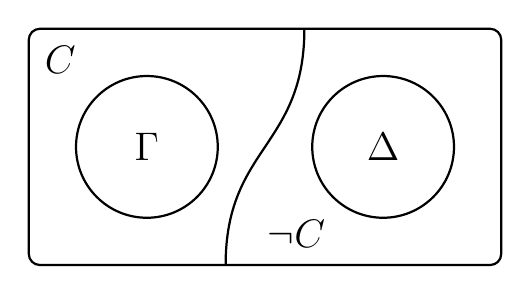
\begin{tikzpicture}[node distance=2cm, auto, thick]
    \draw [rounded corners] (0,0) -- (6,0) -- (6,3) -- (0,3) --  cycle;
    \draw (1.5,1.5) circle (0.9cm);
    \draw (4.5,1.5) circle (0.9cm);
    \path node at (1.5,1.5) {\Large $\Gamma$};
    \path node at (4.5,1.5) {\Large $\Delta$};
    \path node at (0.4,2.6) {\Large $\formula{C}$};
    \path node at (3.4,0.4) {\Large $\lnot \formula{C}$};
    \draw (2.5,0) .. controls (2.5,1.5) and (3.5,1.5) .. (3.5,3);
  \end{tikzpicture}
  \caption{$!C$ 分离 $\Gamma$ 与 $\Delta$}
  \ollabel{fig:sep}
\end{figure}


\begin{lem}\ollabel{lem:sep1}
设 $\Lang{L}_0$ 为包含在 $\Gamma$ 与 $\Delta$ \emph{两者}中均出现的所有常项符号、函数符号及谓词符号（$\doteq$ 除外）的语言，并令 $\Lang{L}'_0$ 为通过添加无穷多个新常项符号 $\Obj c_n$（$n \ge 0$）而得到的语言。那么，如果 $\Gamma$ 与 $\Delta$ 在 $\Lang{L}_0$ 中不可分离，则它们在 $\Lang{L}'_0$ 中也不可分离。
\end{lem}

\begin{proof}
我们反证如下：设 $\Gamma$ 与 $\Delta$ 在 $\Lang{L}'_0$ 中是可分离的。则存在 $!C \in \Lang{L}_0$，使得 $\Gamma \Entails
\Subst{!C}{c}{x}$ 与 $\Delta \Entails \lnot \Subst{!C}{c}{x}$（其中 $c$ 是一个新的常项符号——$!C$ 包含多于一个此类新常项符号的情形是类似的）。由紧致性定理，存在 $\Gamma$ 的有穷子集 $\Gamma_0$ 和 $\Delta$ 的有穷子集 $\Delta_0$，使得 $\Gamma_0 \Entails \Subst{!C}{c}{x}$ 与 $\Delta_0 \Entails \lnot \Subst{!C}{c}{x}$。令 $!G$ 为 $\Gamma_0$ 中所有公式的合取，$!H$ 为 $\Delta_0$ 中所有公式的合取。则
\begin{align*}
  !G & \Entails \Subst{!C}{c}{x}, & !H  \Entails \lnot \Subst{!C}{c}{x}.
\end{align*}
由前者，根据全称概括，得 $!G \Entails
\lforall[x][!C]$；而由后者，通过换质位法，得 $\Subst{!C}{c}{x} \Entails \lnot !H$，从而也有 $\lforall[x][!C]
\Entails \lnot \delta$。再次使用换质位法，得 $!H \Entails
\lnot \lforall[x][!C]$。根据单调性，
\begin{align*}
  \Gamma &\Entails \lforall[x][!C], &
  \Delta & \Entails \lnot \lforall[x][!C],
\end{align*}
因此 $\lforall[x][!C]$ 在 $\Lang{L}_0$ 中分离了 $\Gamma$ 与 $\Delta$。
\end{proof}

\begin{lem}\ollabel{lem:sep2}
假设 $\Gamma \cup \{ \lexists[x][!S] \}$ 与 $\Delta$ 不可分离，且 $c$ 为不在 $\Gamma$、$\Delta$ 或 $!S$ 中出现的新常项符号。则 $\Gamma \cup \{ \lexists[x][!S], \Subst{!S}{c}{x} \}$ 与 $\Delta$ 也是不可分离的。
\end{lem}

\begin{proof}
反设 $!C$ 分离了 $\Gamma \cup \{
\lexists[x][!S], \Subst{!S}{c}{x}\}$ 与 $\Delta$，而 $\Gamma \cup \{\lexists[x]{!S} \}$ 与 $\Delta$ 不可分离。我们区分两种情况：
\begin{enumerate}
\item $c$ 不在 $!C$ 中出现：在这种情况下，$\Gamma \cup
  \{\lexists[x][!S], \lnot!C \}$ 是可满足的（否则 $!C$ 就分离了 $\Gamma \cup \{\lexists[x][!S] \}$ 与 $\Delta$）。加入 $\Subst{!S}{c}{x}$ 后它仍然可满足，所以 $!C$ 并未分离 $\Gamma \cup \{ \lexists[x][!S], \Subst{!S}{c}{x} \}$ 与 $\Delta$。
\item $c$ 在 $!C$ 中出现，从而 $!C$ 具有形式 $\Subst{!C}{c}{x}$。那么我们有
  \[
  \Gamma \cup \{ \lexists[x][!S], \Subst{!S}{c}{x}\} \Entails \Subst{!C}{c}{x},
  \]
  由此，根据演绎定理和全称概括，可得 $\Gamma, \lexists[x][!S] \Entails \lforall[x][(!S \lif !C)]$，最终得到 $\Gamma
  \cup \{ \lexists[x][!S] \} \Entails \lexists[x][!C]$。另一方面，$\Delta \Entails \lnot \Subst{!C}{c}{x}$，进而由全称概括得 $\Delta \Entails \lnot \lexists[x][!C]$。因此 $\Gamma
  \cup \{\lexists[x][!S] \}$ 与 $\Delta$ 可分离，矛盾。
\end{enumerate}
\end{proof}

\end{document}
